
\begin{proof}




































































































Given an arbitrary realization of $P$, each corridor in the realization has $t$ flags and one skinny rhombus. 
The skinny rhombus  has length $\sqrt{1 + \lr{100N}^{-2}}$.
The height of a skinny rhombus in canonical position is $\frac{1}{100N}$.
The obstacle hexagon has height of $ (t+1) \cdot \sqrt{3}$, and the flag is of height $\sqrt{3}$.  
Suppose there are $m+1$ obstacle hexagons and $m$ corridors between two opposing frame hexagons. 
The  $h_\text{max}$ is the following sum:
$$h_\text{max} = (m+1) (t+1) \sqrt{3} + m \lr{\sqrt{3}+ \frac{1}{100N}}$$
This sum is the equal of the distance between two opposing frame hexagons.%; denote it as $h_\text{max}$.
To find a lower bound on of the total height, we examine some qualities of the noncanonical realizations.

\begin{minipage}{\linewidth}
\begin{center}
\includegraphics[width=.9\columnwidth]{graphics/corridorNonCanonical.pdf}
\captionof{figure}{The obstacle hexagon here is in noncanonical position, and showing the side lengths adjacent to $\alpha_i$.}\label{fig:corridorNonCanonical.pdf}
\end{center}
\end{minipage}

The cross section of an arbitrary corridor must have a height of at least $\sqrt{3}$ everywhere. 
%noncanonical corridor must be at least 
Otherwise, a flag would overlap with an obstacle hexagon; it would no longer remain a realization since the height of a flag is $\sqrt{3}$.
In Figure \ref{fig:corridorNonCanonical.pdf}, we illustrate an obstacle hexagon, its upper corridor with the flag that has the hinge to the skinny rhombus.  
The rhombus is hinged at the midpoint of the upper side of the corridor.
The length from a corridor's midpoint to one end of the corridor is $\frac{N}{2}$.
$\gamma_j$ is the angle between $s_j$ and the horizontal axis at the height of the flag ($j = 1,2,\ldots, m$).
The bound of $\gamma_j$ is:
\begin{equation}\label{eqn:alphaBound}
\begin{array}{rcl}
\gamma_j &\leq & \tan^{-1} \lr{
								\frac{
										\sqrt{1+ \lr{	\frac{1}{100N}	}^2}
								}{
										\frac{N}{2}
								}	
							}\\
&=& \tan^{-1} \lr{\frac{2\sqrt{1 + \frac{1}{(100N)^2}}}{N}}\\
&\leq& \frac{2\sqrt{1 + \frac{1}{(100N)^2}}}{N} - \frac{1}{3}\lr{\frac{2\sqrt{1 + \frac{1}{(100N)^2}}}{N}}^3\\
&=&\frac{\lr{6N^2 - 8 - \frac{8}{(100N)^2}}\cdot \sqrt{1 + \frac{1}{(100N)^2}} }{3N^3}
\end{array} 
\end{equation}
Inequality \ref{eqn:alphaBound} uses the first two terms Maclaurin series of $\tan^{-1}$.
From this inequality, it is clear that as $N \rightarrow \infty$, $\gamma_j \rightarrow 0$.




We can now establish the lower bound of $h$. 
The cross section of the corridor must have a minimum height of $\sqrt{3}$ everywhere.
The height of an obstacle polygon in noncanonical position is $(t+1) \cdot \sec \alpha_i \cdot \sqrt{3}$.
%The height of the cross section of an obstacle polygon and   
\begin{eqnarray*}
h_\text{max} = (m+1) (t+1) \sqrt{3} + m \lr{\sqrt{3}+ \frac{1}{100N}}&\geq& \sum_{i = 1}^{m+1} (t+1) \cdot \sec \alpha_i \cdot \sqrt{3} + m \sqrt{3}\\
(m+1) (t+1) \sum_{i = 1}^{m+1} \lr{1 - \sec \alpha_i}&\geq& m \lr{\sqrt{3} - \lr{\sqrt{3}+ \frac{1}{100N}}}\\
\sum_{i = 1}^{m+1} \lr{ \sec \alpha_i - 1} &\leq& \frac{m}{100 N \sqrt{3} (m+1)(t+1) }\\
\sum_{i = 1}^{m+1} \lr{ \lr{1 + \frac{\alpha_i^2}{2}} - 1} &\leq&\frac{m}{100 N \sqrt{3} (m+1)\lr{\lr{2N^3 - 1}+1} }\\
\sum_{i = 1}^{m+1} \frac{\alpha_i^2}{2} &\leq&\frac{m}{200 N^4 (m+1) \sqrt{3} } \\
\sum_{i = 1}^{m+1} \alpha_i^2 &\leq& \frac{m}{100N^4 (m+1) \sqrt{3}}
\end{eqnarray*}
Focusing on the right hand side of the inequality above, we have the following result:
\begin{eqnarray*}
\frac{m}{100N^4 (m+1) \sqrt{3}} &<& \frac{m}{m+1}\\
\frac{1}{100N^4 \sqrt{3}}&<& 1
\end{eqnarray*}

As $N \rightarrow \infty$, $\frac{m}{100N^4 (m+1) \sqrt{3}} \rightarrow 0$ which implies $\sum_{i = 1}^{m+1} \alpha_i^2$ is bounded.  
The number of obstacle hexagons is determined by a polynomial $N(a,b)$ where $a$ is the number of variables in a corresponding Boolean formula and $b$ is the number of clauses in the Boolean formula.
Since $\alpha_i$ is bounded above, then there is a maximal rotation of each obstacle hexagon from canonical position.
Thus every realization of $P$, the obstacle polygons are close to canonical position.



% \begin{minipage}{\linewidth}
% \begin{center}
% 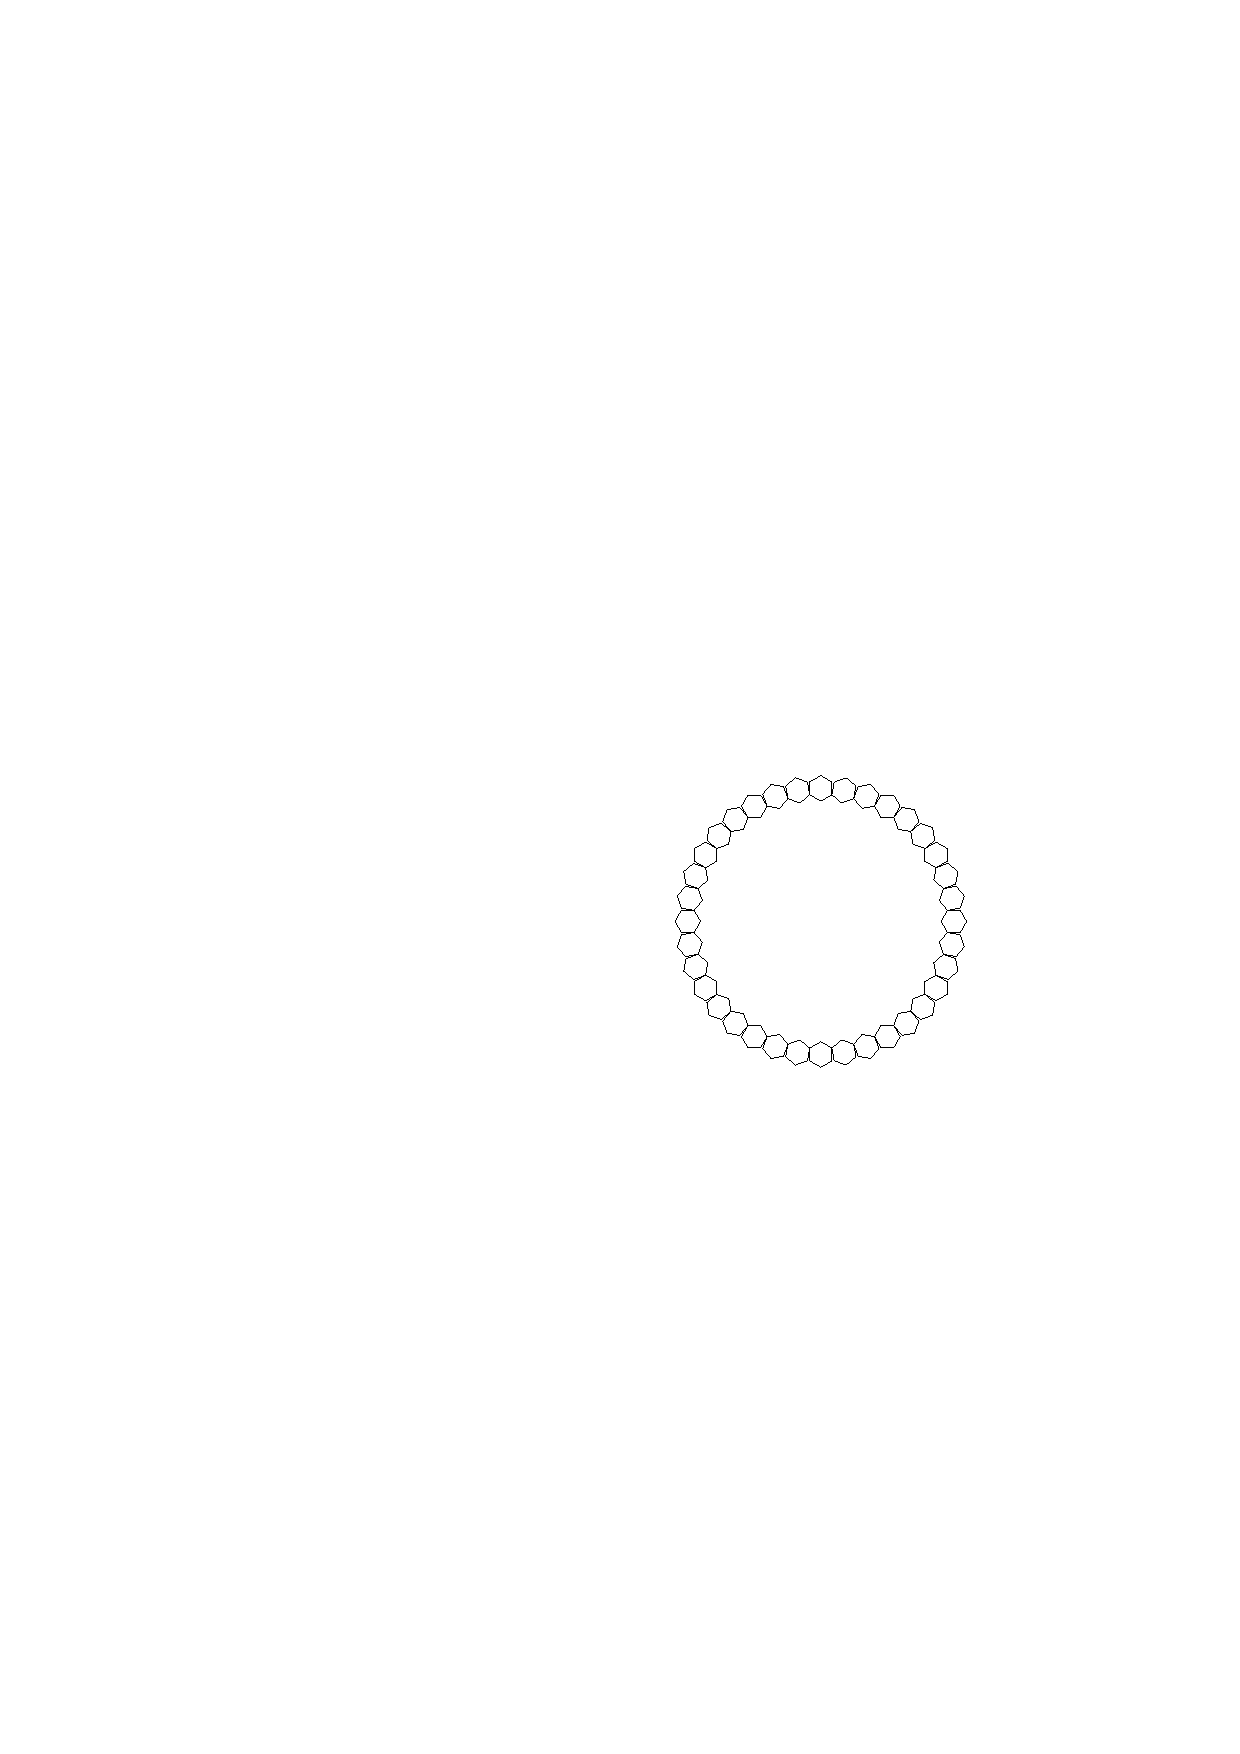
\includegraphics[width=.3\columnwidth]{graphics/WrapAround.pdf}
% \captionof{figure}{This depicts an impossible realization from a column of obstacle hexagons in canonical position to a revolution wrapping around itself.}\label{fig:WrapAround.pdf}
% \end{center}
% \end{minipage}



%1)frame is fixed, only one realization of the frame
%2)NTS that a cross section of a column of obstacle polygons between two opposing hexagon frames
% 	a) h bounds the height
%	b) if alpha_i of the obstacle hexagon is a non-zero angle, the have a larger cross section.
For any realization of P, the frame hexagons are fixed in position.  
This implies there is a fixed height $h$ of any two opposing hexagonal frames.
Suppose we draw a straight line segment $\ell$ of length $h$ from two opposing hexagonal frames; we will use this line segment as a guide to show that the modified auxilary construction admits a realization such that the obstascle polygons along $\ell$ has a maximal displacement from canonical position.
$h$ is the upper bound of the height of vertically aligned obstacle hexagons and corridors.

\begin{minipage}{\linewidth}
\begin{center}
\includegraphics[width=.2\columnwidth ]{graphics/CrossSectionArea.pdf}
\captionof{figure}{The red dashed boxes enclosing the obstacle hexagons in the center column establish the cross sectional area for each obstacle hexagon in canonical position.}\label{fig:CrossSectionArea.pdf}
\end{center}
\end{minipage}

In Figure \ref{fig:CrossSectionArea.pdf}, the cross section of each obstacle hexagon in canonical position denoted in red dashed boxes.
The skinny rhombi attached to flags have freedom to move (see Figure \ref{fig:FlagWithRhombus.pdf}).

\begin{minipage}{\linewidth}
\begin{center}
\includegraphics[width=.33\columnwidth]{graphics/FlagWithRhombus.pdf}
\captionof{figure}{The figure shows the a flag with a skinny rhombus in a corridor.  The red circle shows a potential range of motion of the rhombus.}\label{fig:FlagWithRhombus.pdf}
\end{center}
\end{minipage}

Denote the obstacle hexagons in a column along $\ell$ as $O_1$, $O_2$, $\ldots$, $O_{m+1}$.
% Suppose the realization of P is not in canonical position.
Then there exists some angular rotation for $\alpha_i$ compared to canonical position for each obestacle hexagon $O_i$ for $i = 1 , \ldots, m+1$ (see Figuree \ref{fig:hexagonNonCanonical.pdf}).
If $\alpha_i$ is nonzero, the length of the cross section $\ell \cap O_i$ from $(t+1) \sqrt{3}$ to:% the canonical height of the obstacle hexagon changes from $(t+1) \sqrt{3}$ to:
\begin{eqnarray*}
\text{length}\lr{\ell \cap O_i}=\frac{(t+1) \sqrt{3}}{\cos \alpha_i} &=& (t+1) \cdot \sec \alpha_i \cdot \sqrt{3}\\
&\geq& (t+1) \lr{1 + \frac{\alpha_i^2}{2}} \sqrt{3}\\
&&\text{ where } \frac{-\pi}{2} \leq \alpha_i \leq \frac{\pi}{2}
\end{eqnarray*}
Where we use the fact that the Maclaurin series of $\sec \alpha_i$ expanded to two terms is $\lr{1 + \frac{\alpha_i^2}{2}} $.





% We can now establish the lower bound of $h$. 
% The smallest height of a corridor is $\sqrt{3}$.
% The height of an obstacle polygon in noncanonical position is $(t+1) \cdot \sec \alpha_i \cdot \sqrt{3}$.  
\begin{eqnarray*}
h_\text{max} = (m+1) (t+1) \sqrt{3} + m \lr{\sqrt{3} + \frac{1}{100N}}&\geq& \sum_{i = 1}^{m+1} (t+1) \cdot \sec \alpha_i \cdot \sqrt{3} + m \sqrt{3}\\
%h_\text{max} = m \cdot \lr{\sqrt{3} + 1 + \frac{1}{100N} + (t+1) \cdot \sqrt{3}} + (t+1) \cdot \sqrt{3}  &\geq& \sum_{i = 1}^{m+1} (t+1) \cdot \sec \alpha_i \cdot \sqrt{3} + m \sqrt{3}\\	
%h_\text{max} = m \cdot \lr{\sqrt{3} + 1 + \frac{1}{100N} + (t+1) \cdot \sqrt{3}} + (t+1) \cdot \sqrt{3}  &\geq& \sum_{i = 1}^{m+1} (t+1) \cdot \sec \alpha_i \cdot \sqrt{3} + m \sqrt{3}\\
&\iff&\\
(m+1) (t+1) \sum_{i = 1}^{m+1} \lr{1 - \sec \alpha_i}&\geq& m \lr{\sqrt{3} - \lr{\sqrt{3}+ \frac{1}{100N}}}\\
&\iff&\\
\sum_{i = 1}^{m+1} \lr{ \sec \alpha_i - 1} &\leq& \frac{m}{100 N \sqrt{3} (m+1)(t+1) }\\
\sum_{i = 1}^{m+1}  \sec \alpha_i &\leq& \frac{m}{100 N \sqrt{3} (m+1)(t+1) } + (m+1)
\end{eqnarray*}
% The bound above shows that each $\alpha_i$ is bounded above by the right hand side, i.e.:
% \begin{equation}\label{eqn:alphaBound}
% \alpha_i \leq \sec^{-1} \lr{\frac{m}{100 N \sqrt{3} (m+1)(t+1) } + (m+1)}
% \end{equation}
% Since $\alpha_i$ is bounded above, then there is a maximal rotation of each obstacle hexagon from canonical position.
% Thus every realization of $P$, the obstacle polygons are close to canonical position.
% %Let P be a polygonal linkage obtained from the modified auxilary construction.  
% % In every realization of $P$, the obstacle polygons are close to canonical position.



% Since the angles $\alpha_i$ are so small, extreme configurations of obstacle hexagons like the spiral in Figure \ref{fig:WrapAround.pdf} are not feasible.























































































































\end{proof}